\documentclass[12pt]{article}

\usepackage[utf8]{inputenc}


%% packages
\usepackage{color,verbatim,Sweave,url,xargs,amsmath,hyperref,booktabs,longtable}
\usepackage[left=2cm,right=2cm,top=2cm,bottom=2cm]{geometry}

%% new environments
\newenvironment{question}{\item \textbf{Problem}\newline}{}
\newenvironment{solution}{\textbf{Solution}\newline}{\newpage}
\newenvironment{answerlist}{\renewcommand{\labelenumi}{(\alph{enumi})}\begin{enumerate}}{\end{enumerate}}

%% paragraphs
\setlength{\parskip}{0.7ex plus0.1ex minus0.1ex}
\setlength{\parindent}{0em}

%% compatibility with pandoc
\providecommand{\tightlist}{\setlength{\itemsep}{0pt}\setlength{\parskip}{0pt}}

%% fonts: Helvetica
\renewcommand{\sfdefault}{phv}
\IfFileExists{sfmath.sty}{
  \RequirePackage[helvet]{sfmath}
  \renewcommand{\rmdefault}{phv}
}{}

\newcommand{\extext}[1]{\textbf{\large #1}}
\newcommandx{\exmchoice}[9][2=-,3=-,4=-,5=-,6=-,7=-,8=-,9=-]{%
                \mbox{(a) \,\, \framebox[8mm]{\rule[-1mm]{0mm}{5mm} \hspace*{-1.6mm} \extext{#1}} \hspace*{2mm}}%
  \if #2- \else \mbox{(b) \,\, \framebox[8mm]{\rule[-1mm]{0mm}{5mm} \hspace*{-1.6mm} \extext{#2}} \hspace*{2mm}} \fi%
  \if #3- \else \mbox{(c) \,\, \framebox[8mm]{\rule[-1mm]{0mm}{5mm} \hspace*{-1.6mm} \extext{#3}} \hspace*{2mm}} \fi%
  \if #4- \else \mbox{(d) \,\, \framebox[8mm]{\rule[-1mm]{0mm}{5mm} \hspace*{-1.6mm} \extext{#4}} \hspace*{2mm}} \fi%
  \if #5- \else \mbox{(e) \,\, \framebox[8mm]{\rule[-1mm]{0mm}{5mm} \hspace*{-1.6mm} \extext{#5}} \hspace*{2mm}} \fi%
  \if #6- \else \mbox{(f) \,\, \framebox[8mm]{\rule[-1mm]{0mm}{5mm} \hspace*{-1.6mm} \extext{#6}} \hspace*{2mm}} \fi%
  \if #7- \else \mbox{(g) \,\, \framebox[8mm]{\rule[-1mm]{0mm}{5mm} \hspace*{-1.6mm} \extext{#7}} \hspace*{2mm}} \fi%
  \if #8- \else \mbox{(h) \,\, \framebox[8mm]{\rule[-1mm]{0mm}{5mm} \hspace*{-1.6mm} \extext{#8}} \hspace*{2mm}} \fi%
  \if #9- \else \mbox{(i) \,\, \framebox[8mm]{\rule[-1mm]{0mm}{5mm} \hspace*{-1.6mm} \extext{#9}} \hspace*{2mm}} \fi%
}
\newcommandx{\exclozechoice}[9][2=-,3=-,4=-,5=-,6=-,7=-,8=-,9=-]{\setcounter{enumiii}{1}%
                \mbox{\roman{enumiii}. \, \framebox[8mm]{\rule[-1mm]{0mm}{5mm} \hspace*{-1.6mm} \extext{#1}} \hspace*{2mm}\stepcounter{enumiii}}%
  \if #2- \else \mbox{\roman{enumiii}. \, \framebox[8mm]{\rule[-1mm]{0mm}{5mm} \hspace*{-1.6mm} \extext{#2}} \hspace*{2mm}\stepcounter{enumiii}} \fi%
  \if #3- \else \mbox{\roman{enumiii}. \, \framebox[8mm]{\rule[-1mm]{0mm}{5mm} \hspace*{-1.6mm} \extext{#3}} \hspace*{2mm}\stepcounter{enumiii}} \fi%
  \if #4- \else \mbox{\roman{enumiii}. \, \framebox[8mm]{\rule[-1mm]{0mm}{5mm} \hspace*{-1.6mm} \extext{#4}} \hspace*{2mm}\stepcounter{enumiii}} \fi%
  \if #5- \else \mbox{\roman{enumiii}. \, \framebox[8mm]{\rule[-1mm]{0mm}{5mm} \hspace*{-1.6mm} \extext{#5}} \hspace*{2mm}\stepcounter{enumiii}} \fi%
  \if #6- \else \mbox{\roman{enumiii}. \, \framebox[8mm]{\rule[-1mm]{0mm}{5mm} \hspace*{-1.6mm} \extext{#6}} \hspace*{2mm}\stepcounter{enumiii}} \fi%
  \if #7- \else \mbox{\roman{enumiii}. \, \framebox[8mm]{\rule[-1mm]{0mm}{5mm} \hspace*{-1.6mm} \extext{#7}} \hspace*{2mm}\stepcounter{enumiii}} \fi%
  \if #8- \else \mbox{\roman{enumiii}. \, \framebox[8mm]{\rule[-1mm]{0mm}{5mm} \hspace*{-1.6mm} \extext{#8}} \hspace*{2mm}\stepcounter{enumiii}} \fi%
  \if #9- \else \mbox{\roman{enumiii}. \, \framebox[8mm]{\rule[-1mm]{0mm}{5mm} \hspace*{-1.6mm} \extext{#9}} \hspace*{2mm}} \fi%
}
\newcommand{\exnum}[9]{%
  \mbox{\framebox[8mm]{\rule[-1mm]{0mm}{5mm} \hspace*{-1.6mm} \extext{#1}}}%
  \mbox{\framebox[8mm]{\rule[-1mm]{0mm}{5mm} \hspace*{-1.6mm} \extext{#2}}}%
  \mbox{\framebox[8mm]{\rule[-1mm]{0mm}{5mm} \hspace*{-1.6mm} \extext{#3}}}%
  \mbox{\framebox[8mm]{\rule[-1mm]{0mm}{5mm} \hspace*{-1.6mm} \extext{#4}}}%
  \mbox{\framebox[8mm]{\rule[-1mm]{0mm}{5mm} \hspace*{-1.6mm} \extext{#5}}}%
  \mbox{\framebox[8mm]{\rule[-1mm]{0mm}{5mm} \hspace*{-1.6mm} \extext{#6}}}%
  \mbox{ \makebox[3mm]{\rule[-1mm]{0mm}{5mm} \hspace*{-2mm} .}}%
  \mbox{\framebox[8mm]{\rule[-1mm]{0mm}{5mm} \hspace*{-1.6mm} \extext{#7}}}%
  \mbox{\framebox[8mm]{\rule[-1mm]{0mm}{5mm} \hspace*{-1.6mm} \extext{#8}}}%
  \mbox{\framebox[8mm]{\rule[-1mm]{0mm}{5mm} \hspace*{-1.6mm} \extext{#9}}}%
}
\newcommand{\exstring}[1]{%
  \mbox{\framebox[0.9\textwidth][l]{\rule[-1mm]{0mm}{5mm} \hspace*{-1.6mm} \extext{#1}} \hspace*{2mm}}%
}

%% new commands
\makeatletter
\newcommand{\ID}[1]{\def\@ID{#1}}
\newcommand{\Date}[1]{\def\@Date{#1}}
\ID{00001}
\Date{YYYY-MM-DD}

\Date{2019-04-25}
\ID{055}

\newcommand{\myID}{\@ID}
\newcommand{\myDate}{\@Date}
\makeatother

%% headings
\markboth{\textnormal{\bf \large \textsc{Mat-181 3rd Exam}, version \myID}}%
{\textnormal{\bf \large Mat-181 3rd Exam, version \myID, NO OUTSIDE HELP}}
\pagestyle{myheadings}

\begin{document}

%% title page
\thispagestyle{empty}
{\sf
\textbf{\LARGE{Bunker Hill Community College}}



\textbf{\large{Third Statistics Exam \myDate \hfill Exam ID \myID}}

\vspace*{2cm}

\begin{center}
\begin{tabular}{p{16cm}}
\textbf{Name:} ANSWER KEY \hrule \\[1.5cm]
\end{tabular}
\end{center}

This take-home exam is due {\bf Monday, April 29} at the beginning of class.

You may use any notes, textbook, or online tools; however, you may not request help from any other human. If you believe a question is ambiguous, unanswerable, or erroneous, please let me know.

You will show your work on the pages with questions. When you are sure of your answers, you will put those answers in the boxes on the first few pages.

Unless you have an objection to doing so, please copy the honor-code text below and sign. 

\vspace{20pt}
\begin{center}
\emph{I understand that outside help is NOT allowed on this exam. On my honor, the work herein is my own.}
\end{center}

\vspace{1.5cm}
\begin{center}
\begin{tabular}{p{16cm}}
\hrule  \\[1.5cm]
\hrule  \\[1.5cm]
\hrule  \\[1.5cm]
\textbf{Signature:} \hrule  \\[1.5cm]
\end{tabular}
\end{center}

\newpage

\begin{enumerate}
  \item 
   \begin{enumerate}
      \item \exstring{LB = 14.8}\\
      \item \exstring{UB = 15.5} 
  \end{enumerate}
  \item 
   \begin{enumerate}
      \item \exstring{$H_0: \mu_\text{diff}=0$}\\
      \item \exstring{$H_\text{A}: \mu_\text{diff} \ne 0$}\\
      \item \exstring{$t^\star = 1.94$}\\
      \item \exstring{$SE = 1.36$}\\
      \item \exstring{$\mid t_\text{obs}\mid = 2.103$}\\
      \item \exstring{$0.05 < p\text{-value} < 0.1$}\\
      \item \exstring{reject} 
  \end{enumerate}
  \item 
   \begin{enumerate}
      \item \exstring{$H_0:~~\mu_2-\mu_1 = 0$}\\
      \item \exstring{$H_0:~~\mu_2-\mu_1 \ne 0$}\\
      \item \exstring{$t^\star = 2.57$}\\
      \item \exstring{$SE = 52$}\\
      \item \exstring{$\mid t_\text{obs}\mid = 2.31$}\\
      \item \exstring{$0.05 < p\text{-value} < 0.1$}\\
      \item \exstring{retain} 
  \end{enumerate}
  \item 
   \begin{enumerate}
      \item \exstring{LB of p CI = 0.17 or $17\%$}\\
      \item \exstring{UB of p CI = 0.24 or $24\%$} 
  \end{enumerate}
  \item \exstring{$n \approx 31000$}
  \item 
   \begin{enumerate}
      \item \exstring{$H_0: ~~p_2-p_1=0$}\\
      \item \exstring{$H_\text{A}:~~ p_2-p_1\ne 0$}\\
      \item \exstring{$z^\star = 1.64$}\\
      \item \exstring{$SE=0.036$}\\
      \item \exstring{$\mid z_\text{obs} \mid=1.85$}\\
      \item \exstring{$p\text{-value} = 0.0644$}\\
      \item \exstring{reject} 
  \end{enumerate}
\end{enumerate}

}
\newpage

\begin{enumerate}


\begin{question}
An experiment has \(n_1 = 4\) plants in the treatment group and
\(n_2 = 6\) plants in the control group. After some time, the plants'
heights (in cm) are measured, resulting in the following data:

\begin{longtable}[]{@{}ccccccc@{}}
\toprule
& value1 & value2 & value3 & value4 & value5 & value6\tabularnewline
\midrule
\endhead
sample 1: & 16.4 & 14.2 & 19.4 & 17.3\tabularnewline
sample 2: & 10.3 & 9.9 & 9.4 & 11 & 10.4 & 10.7\tabularnewline
\bottomrule
\end{longtable}
\begin{answerlist}
  \item Determine degrees of freedom.
  \item Determine \(t^\star\) for a \(98\%\) confidence interval.
  \item Determine \(SE\).
  \item Determine a lower bound of the \(98\%\) confidence interval of
\(\mu_2-\mu_1\).
  \item Determine an upper bound of the \(98\%\) confidence interval of
\(\mu_2-\mu_1\).
  \item Determine \(|t_\text{obs}|\) under the null hypothesis
\(\mu_2-\mu_1=0\).
  \item Determine a lower bound of the two-tail \(p\)-value.
  \item Determine an upper bound of two-tail \(p\)-value.
  \item Do you reject the null hypothesis with a two-tail test using a
significance level \(\alpha = 0.02\)? (yes or no)
\end{answerlist}
\end{question}

\begin{solution}
These data are unpaired. We might as well find the sample means and
sample standard deviations (use a calculator's built-in function for
standard deviation). \[\overline{x_1} = 16.8 \]
\[\overline{x_2} = 10.3 \] \[s_1 = 2.15 \] \[s_2 = 0.571 \]

We make a conservative estimate of the degrees of freedom using the
appropriate formula. \[df ~=~ \min(n_1,\,n_2)-1 ~=~ \min(4,6)-1 ~=~ 3 \]
We use the \(t\) table to find \(t^\star\) such that
\(P(|T|<t^\star) = 0.98\) \[t^\star = 4.54 \] We use the \(SE\) formula
for unpaired data.
\[SE = \sqrt{\frac{(s_1)^2}{n_1}+\frac{(s_2)^2}{n_2}} =
\sqrt{\frac{(2.15)^2}{4}+\frac{(0.571)^2}{6}} = 1.1 \] We find the
bounds of the confidence interval.
\[CI ~=~ (\overline{x_2}-\overline{x_1})\pm t^{\star} SE\]
\[CI ~=~ (-11.494,\, -1.506) \] We find \(t_\text{obs}\).
\[t_\text{obs} = \frac{(\overline{x_2}-\overline{x_1})-(\mu_2-\mu_1)_0}{SE} = \frac{(10.3-16.8)-0}{1.1} = -5.91\]
We find \(|t_\text{obs}|\). \[|t_\text{obs}| = 5.91 \] We use the table
to determine bounds on \(p\)-value. Remember, \(df=3\) and
\(p\text{-value} = P(|T|>|t_\text{obs}|)\).
\[0.005 ~<~ p\text{-value} ~<~ 0.01\] We should consider both
comparisons to make our decision. \[|t_\text{obs}| > t^{\star} \]
\[p\text{-value} < \alpha \] Thus, we reject the null hypothesis. Also
notice the confidence interval does not contain 0.
\begin{answerlist}
  \item 3
  \item 4.54
  \item 1.1
  \item -11.494
  \item -1.506
  \item 5.909
  \item 0.005
  \item 0.01
  \item yes
\end{answerlist}
\end{solution}



\begin{question}
In a deck of strange cards, each card has an image and a color. The
chance of drawing a gem is 45.1\%. If a gem is drawn, there is a 87\%
chance that it is red. If a card that is not a gem is drawn, there is a
21.5\% chance that it is red.

Now, someone draws a random card and reveals it is red. What is the
chance the card is not a gem?
\end{question}

\begin{solution}
I'd recommend making a tree. Remember, on the first branch, we put
simple probabilities. On the second branches we put conditional
probabilites. The results (products) are joint probabilities.

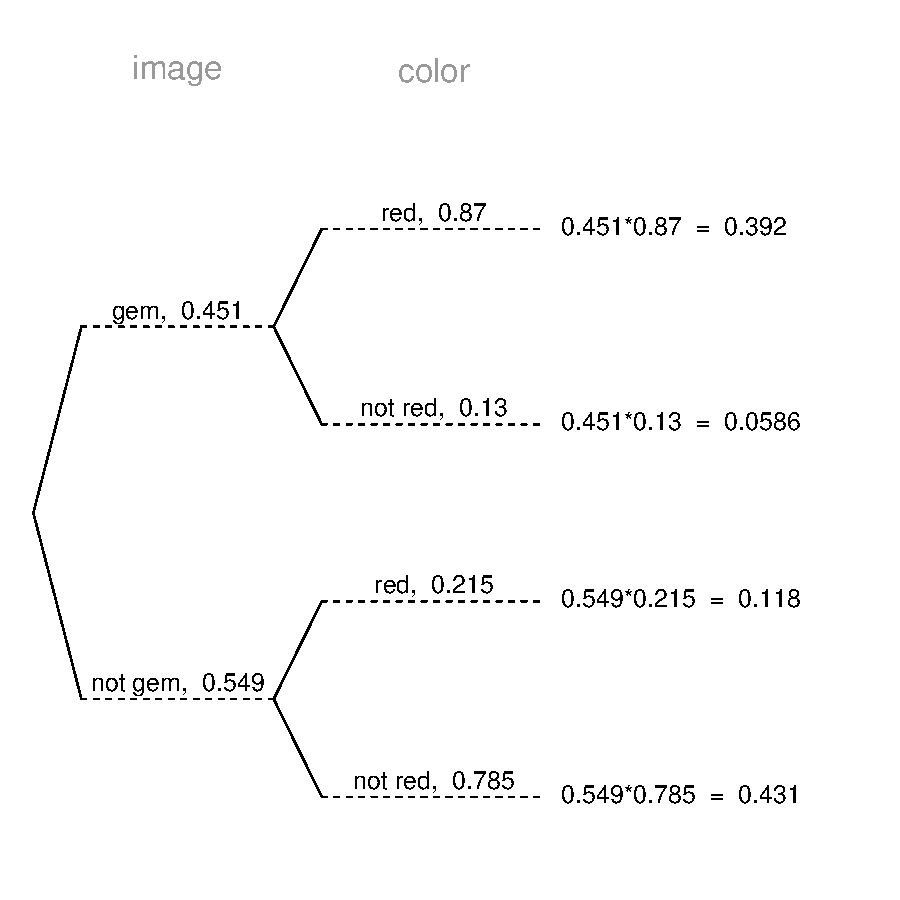
\includegraphics{tree-1.pdf} ~

Determine the appropriate conditional probability.
\[P(\text{"not gem" given "red"}) = \frac{0.118}{0.118+0.392} = 0.231 \]
\end{solution}



\begin{question}
In a very large pile of toothpicks, the mean length is 65.72 millimeters
and the standard deviation is 3.84 millimeters. If you randomly sample
169 toothpicks, what is the chance the sample mean is between 64.96 and
65.89 millimeters?
\end{question}

\begin{solution}
Label the given information. \[ 
\begin{aligned}
\mu &= 65.72\\
\sigma &= 3.84\\
n &= 169\\
\bar{x}_\text{lower} &= 64.96 \\
\bar{x}_\text{upper} &= 65.89
\end{aligned}
\] Find the standard error.
\[SE = \frac{\sigma}{\sqrt{n}} = \frac{3.84}{\sqrt{169}} = 0.295 \]
Describe the sampling distribution.
\[\bar{X} \sim \mathcal{N}(65.72,\,0.295) \]

Draw a sketch.\\
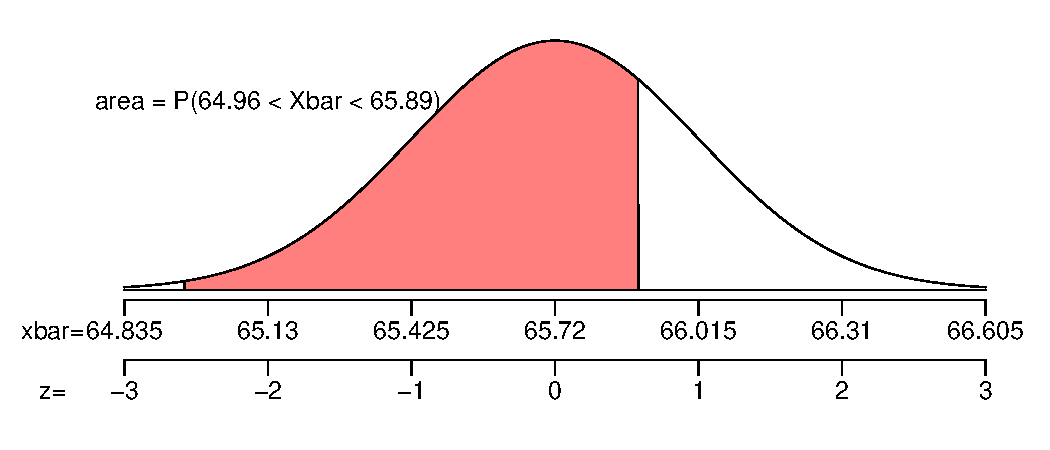
\includegraphics{normal_sketch_sampling-1.pdf} ~

Calculate a \(z\) scores.
\[z_\text{lower} = \frac{x_\text{lower}-\mu}{SE} = \frac{64.96-65.72}{0.295} = -2.58 \]
\[z_\text{upper} = \frac{x_\text{upper}-\mu}{SE} = \frac{65.89-65.72}{0.295} = 0.58 \]
Determine the probability. \[
\begin{aligned}
P(64.96 < X < 65.89) &= \Phi(z_\text{upper}) - \Phi(z_\text{lower}) \\
&= \Phi(0.58) - \Phi(-2.58) \\
&= 0.7141 
\end{aligned}
\]
\end{solution}



\begin{question}
From a very large population, a random sample of 550 individuals was
taken. In that sample, 20.5\% were asleep. Determine a 96\% confidence
interval of the population proportion.
\begin{answerlist}
  \item Find the lower bound of the confidence interval.
  \item Find the upper bound of the condifence interval.
\end{answerlist}
\end{question}

\begin{solution}
Determine \(z^\star\) such that \(P(|Z|<z^\star) = 0.96\).
\[z^\star = 2.05 \] Calculate the standard error.
\[SE = \sqrt{\frac{\hat{p}(1-\hat{p})}{n}} = \sqrt{\frac{(0.205)(1-0.205)}{550}} = 0.0172 \]
Calculate the margin of error.
\[ME = z^\star SE = (2.05)(0.0172) = 0.0353 \] To find the confidence
interval's bounds, find the sample proportion plus or minus the margin
of error. \[p ~\approx~ \hat{p} \pm ME \] Determine the interval.
\[(0.17\,,~ 0.24) \] We are 96\% confident that the true population
proportion is between 17\% and 24\%.
\begin{answerlist}
  \item The lower bound = 0.17, which can also be expressed as 17\%.
  \item The upper bound = 0.24, which can also be expressed as 24\%.
\end{answerlist}
\end{solution}



\begin{question}
As an ornithologist, you wish to determine the average body mass of
\emph{Piranga rubra}. You randomly sample 31 adults of \emph{Piranga
rubra}, resulting in a sample mean of 37.46 grams and a sample standard
deviation of 6.73 grams. Determine a 99.5\% confidence interval of the
true population mean.
\end{question}

\begin{solution}
We are given the sample size, sample mean, sample standard deviation,
and confidence level. \[
\begin{aligned}
n &= 31 \\
\bar{x} &= 37.46 \\
s &= 6.73\\
CL &= 0.995
\end{aligned}
\] Determine the degrees of freedom (because we don't know \(\sigma\)
and we are doing inference so we need to use the \(t\) distribution).
\[df = n-1 = 30\] Determine the critical \(t\) value, \(t^\star\), such
that \(P(|T|<t^\star) = 0.995\). \[t^\star = 3.03 \] Calculate the
standard error.
\[ SE = \frac{s}{\sqrt{n}} = \frac{6.73}{\sqrt{31}} = 1.21 \] We want to
make an inference about the population mean.
\[\mu ~\approx~ \bar{x}\pm t^\star SE \] Determine the bounds. \[
\begin{aligned}
CI &= (\bar{x} - t^\star SE,\,\bar{x} + t^\star SE) \\
   &= (37.46 - 3.03\times1.21,\,37.46 + 3.03\times1.21) \\
   &= (33.8,\,41.1) 
\end{aligned}
\] We are 99.5\% confident that the population mean is between 33.8 and
41.1.
\end{solution}



\begin{question}
A random sample of size 66000 was found to have a sample proportion of
6.4\%. Determine a 90\% confidence interval of the population
proportion.
\begin{answerlist}
  \item Find the lower bound of the confidence interval.
  \item Find the upper bound of the condifence interval.
\end{answerlist}
\end{question}

\begin{solution}
Determine \(z^\star\) such that \(P(|Z|<z^\star) = 0.9\).
\[z^\star = 1.64 \] Calculate the standard error.
\[SE = \sqrt{\frac{\hat{p}(1-\hat{p})}{n}} = \sqrt{\frac{(0.064)(1-0.064)}{66000}} = 0.000953 \]
Calculate the margin of error.
\[ME = z^\star SE = (1.64)(0.000953) = 0.00156 \] To find the confidence
interval's bounds, find the sample proportion plus or minus the margin
of error. \[p ~\approx~ \hat{p} \pm ME \] Determine the interval.
\[(0.0624\,,~ 0.0656) \] We are 90\% confident that the true population
proportion is between 6.24\% and 6.56\%.
\begin{answerlist}
  \item The lower bound = 0.0624, which can also be expressed as 6.24\%.
  \item The upper bound = 0.0656, which can also be expressed as 6.56\%.
\end{answerlist}
\end{solution}



\end{enumerate}

\end{document}
